% ====================================================================
% Paper 4 — Topological Pathology: Disease as Impedance Failure
% ====================================================================
\documentclass[aps,pre,twocolumn,superscriptaddress,floatfix]{revtex4-2}
\usepackage{amsmath,amssymb,amsthm}
\usepackage{graphicx}
\usepackage{hyperref}
\usepackage{float}
\usepackage{booktabs}
\usepackage{gammanet}

\begin{document}

\title{Paper~4: Topological Pathology\\
--- Disease as Impedance Failure\\
on the $\Gamma$-Network}

\author{Hsi-Yu Huang}
\email{llc.y.huangll@gmail.com}
\affiliation{Independent Researcher, Taipei, Taiwan}

\date{\today}

\begin{abstract}
Papers~1--3 of this series developed the spatial
(irreducibility, dual-network scaling) and temporal
(impedance debt, sleep, lifecycle, remodeling)
architecture of impedance-minimising networks.
Here we show that \emph{disease}---from single-organ
pathology to multi-organ failure---emerges as a
direct consequence of impedance physics on these
networks, without any disease-specific code.

\textbf{Part~A} demonstrates that neural pathology is
determined by network topology:
stroke (edge severance), ALS (impedance escalation),
neurodegeneration (mode loss), and pain (high-$\Gamma$
signal on low-$K$ pathways) all follow from the
irreducibility theorem (Paper~1) and C2
gradient descent.

\textbf{Part~B} derives the dual-network disease cascade:
a five-step positive-feedback loop
($\Gamma_v\!\uparrow \to \rho\!\downarrow \to
\Gamma_n\!\uparrow \to \text{autonomic}\!\downarrow
\to \Gamma_v\!\uparrow\!\uparrow$) that drives
vascular--neural co-failure.
We instantiate this cascade for atherosclerosis,
aneurysm, diabetic microvascular disease, vascular
dementia, and pre-eclampsia, and derive wound repair
as spatial impedance matching with a health index
$H_{\text{wound}} = (1-\Gamma_n^2)(1-\Gamma_v^2)$.

\textbf{Part~C} formalises the coupled multi-organ
dynamics:
$d\Gamma_k^2/dt$ for five organ channels with
inter-channel coupling, positive feedback,
and aging damage.
Disease onset is a saddle-node bifurcation (phase
transition); recovery depends on whether zero, one,
or multiple channels have crossed their thresholds.
We derive tissue necrosis as thermodynamic substrate
collapse ($\Gamma = 1$ irreversibly), surgical
intervention as topological truncation,
the caregiver triple-load model, surface
observability (skin as impedance readout),
obesity as impedance-driven metabolic strategy,
type~2 diabetes as a six-channel hexagonal deadlock
(Theorem~\ref{thm:t2d-treatment}),
and the immune--metabolic inflammation--insulin trap.

\textbf{Part~D} proves E0 emergence: clinical pathology
arises from C1/C2/C3 plus initial conditions alone---no
disease-specific flags---across cardiovascular,
neural, thermal, and sleep-disorder domains
(275 automated E0 tests, 100\% pass).

Together, Parts~A--D establish that pathology is not
an external overlay on physiology but a
\emph{necessary consequence} of
$\mathcal{A}[\Gamma] \to \min$ when the network is
perturbed beyond its repair capacity.
\end{abstract}

\maketitle


% %%%%%%%%%%%%%%%%%%%%%%%%%%%%%%%%%%%%%%%%%%%%%%%%%%%%%%%%%%%%
%  PART A — NEURAL PATHOLOGY FROM TOPOLOGY
% %%%%%%%%%%%%%%%%%%%%%%%%%%%%%%%%%%%%%%%%%%%%%%%%%%%%%%%%%%%%
\bigskip\noindent\textbf{\large Part A: Neural Pathology from Topology}
\label{part:A}
\bigskip


\section{Introduction}
\label{sec:intro}

The preceding papers derived the architecture of
impedance-minimising biological networks:
Paper~0 established the framework
(Minimum Reflection Principle, C1/C2/C3);
Paper~1 proved the irreducibility theorem
($A = A_{\text{imp}} + A_{\text{cut}}$) and the
emergence of brain architecture;
Paper~2 derived dual neural--vascular scaling and
organ health $H = (1-\Gamma_n^2)(1-\Gamma_v^2)$;
Paper~3 developed temporal dynamics (impedance debt,
sleep, lifecycle, aging) and proved C2 universality
across twenty-nine tissue-update mechanisms.

All of these results describe \emph{healthy} or
\emph{repairing} systems---networks evolving toward
lower $\Gamma^2$.
This paper asks: what happens when the perturbation
exceeds the repair capacity?
When C2 cannot compensate, when bifurcation thresholds
are crossed, when substrate is destroyed?

The answer is: \emph{disease}.
We show that every major class of pathology---neural,
vascular, metabolic, immune, renal---is a specific
instance of impedance failure on the $\Gamma$-network.
No disease-specific code is needed;
the ``disease'' is the perturbation, and the clinical
pattern is the resulting $\Gamma$-distribution.


\section{Neural Pathology from Topology}
\label{sec:neural-pathology}

The irreducibility theorem (Paper~1) has a direct
clinical implication: because $A_{\text{cut}}$ is
determined by topology (mode counts and edge structure)
and has zero gradient with respect to impedance,
C2 cannot compensate for topological damage.

This establishes a fundamental asymmetry:
\begin{itemize}
  \item \textbf{Impedance perturbation}
    (soft tissue injury, inflammation, transient chemical
    imbalance): C2 can repair, because $A_{\text{imp}}$
    is learnable.
    Given time, $\Gamma_k \to 0$ on the perturbed edges.
  \item \textbf{Topological perturbation}
    (neuron death, axon severance, dendrite retraction):
    C2 cannot repair, because the change affects
    $A_{\text{cut}}$, which is invisible to the gradient.
\end{itemize}

\noindent
This is why brain damage is often permanent while soft
tissue heals.

\begin{theorem}[Neural deficit as topological signature]
\label{thm:neural-topology}
Let $\mathcal{G} = (V, E, K)$ be a neural
\texttt{GammaTopology} with node set $V$,
edge set $E$, and modal complexity assignments $K$.
A topological perturbation $\delta\mathcal{G}$
(edge severance, impedance escalation, or mode loss)
produces a deficit pattern $D(\delta\mathcal{G})$
determined solely by the structural change to
$(V, E, K)$, not by the identity of the affected node.
\end{theorem}

\begin{proof}
The deficit pattern is defined as the set of
transmission paths whose $T_i = 1 - \Gamma_i^2$
falls below clinical threshold after perturbation.
By C3, $\Gamma_i$ at each interface is computable
from local $(Z_{\text{source}}, Z_{\text{load}})$
pairs alone.
Therefore the propagation of any perturbation
through the network is determined entirely by
the topology $(V, E, K)$ and the C2 update rule---
not by the specific molecular identity of the
perturbed node.
Two perturbations that produce identical changes
to $(V, E, K)$ produce identical deficit patterns. $\square$
\end{proof}


\subsection{Edge severance (stroke)}
\label{sec:stroke}

Removing an edge $i \to j$ eliminates a pathway.
Signals that traversed this edge are interrupted.
C2 can strengthen alternative pathways if they exist
(redundancy allows partial recovery), but the lost
edge's contribution to the network is permanently gone.
The deficit pattern is determined by \emph{which edge}
is lost: topology dictates which functions are impaired.


\subsection{Impedance escalation (ALS, demyelination)}
\label{sec:als}

A diseased neuron's impedance $Z$ increases
progressively.
At each of its edges, $\Gamma$ increases and $T$
decreases.
C2 attempts to compensate on neighbouring edges, but if
the disease is progressive ($Z$ continues to rise),
compensation cannot keep pace: the damaged node acts as
a growing impedance barrier that eventually isolates
itself from the network.

The neural topology test confirms this: ALS
(motor neuron $Z \times 3$) produces cumulative
$A_{\text{imp}}$ over 30~ticks that is $2.9\times$
the healthy baseline, with descending motor signals
progressively degraded while sensory pathways remain
intact---matching the clinical pattern.


\subsection{Mode loss (neurodegeneration)}
\label{sec:mode-loss}

A neuron that loses physical structure (spine
retraction, dendrite pruning) loses modes:
$K_i$ decreases.
Previously matched edges (where $K_i = K_j$) now
have $A_{\text{cut}} > 0$.
This new irreducible cost appears abruptly and cannot
be removed by C2.
Cognitive decline is the progressive accumulation of
irreducible cost as neurons lose modes throughout the
convergence region.


\subsection{Pain as $\Gamma$-signal on low-$K$ pathways}
\label{sec:pain-signal}

Tissue damage produces an abrupt local impedance
change, generating a $\Gamma$ spike on nociceptor edges.
Nociceptors sit at the lowest $K$ levels in the
hierarchy (C-fibre $K = 1$, A$\delta$ $K = 2$).
The $\Gamma$ spike propagates through the relay chain
to the convergence region.
Pain is not a special signal type---it is a
high-$\Gamma$ event on a low-$K$ pathway.
Full treatment: Paper~1, Sec.~10~\cite{Paper1}.


\subsection{Stroke verification}
\label{sec:stroke-verify}

The neural topology test confirms that severing the
cortex$\to$thalamus edge interrupts descending motor
transmission while the ascending sensory pathway
remains intact---the topology determines the deficit
pattern without any disease-specific code.


\section{Neural Control Priority Theorem}
\label{sec:neural-control-priority}

The preceding subsections treat neural pathology as a
collection of local topological events.
Here we establish a deeper structural result: because the
neural network is the \emph{control layer} of the entire
$\Gamma$-Net, its failure is not merely one disease among
many---it is the necessary precursor to system-wide
pathological emergence.

\begin{theorem}[Neural Control Priority]
\label{thm:neural-control-priority}
Let $\mathcal{G} = \mathcal{G}_n \cup \mathcal{G}_v \cup
\mathcal{G}_m$ be a $\Gamma$-Net partitioned into neural
($n$), vascular ($v$), and metabolic ($m$) sub-networks,
where $\mathcal{G}_n$ acts as the control layer: each
non-neural node $k \notin \mathcal{G}_n$ receives a
C2 correction signal $\Delta Z_k$ gated by the
transmission $T_{n \to k} = 1 - \Gamma_{n \to k}^2$
along the neural pathway connecting to $k$.

Suppose the system satisfies C1
($\Gamma_k^2 + T_k = 1$ for all $k$) at $t = 0$.
If the neural sub-network suffers a perturbation such
that $\Gamma_{n \to k}^2 > \Gamma_{\mathrm{thr}}^2$ for
some threshold $\Gamma_{\mathrm{thr}} < 1$, then:
\begin{enumerate}
  \item[(i)] The effective C2 update available to every
    non-neural node $k$ is reduced to
    $|\Delta Z_k^{\mathrm{eff}}| \leq
    (1 - \Gamma_{\mathrm{thr}}^2)\,|\Delta Z_k^{\mathrm{max}}|$.
  \item[(ii)] If $|\Delta Z_k^{\mathrm{eff}}|$ falls below
    the minimum correction required to maintain C1 at
    node $k$, then $\Gamma_k^2$ begins to grow
    monotonically.
  \item[(iii)] Consequently, neural failure is a
    \emph{necessary condition} for uncorrectable
    system-wide impedance escalation: no non-neural
    node can lose C1 stability while the neural control
    layer transmits with $\Gamma_{n \to k}^2 \leq
    \Gamma_{\mathrm{thr}}^2$.
\end{enumerate}
\end{theorem}

\begin{proof}
By the C2 update rule (Paper~0), the impedance
correction at node $k$ at each time step is
\begin{equation}
  \Delta Z_k = -\eta\,\Gamma_k\,x_{\mathrm{in},k}\,x_{\mathrm{out},k},
  \label{eq:c2-update}
\end{equation}
where $x_{\mathrm{in},k}$ and $x_{\mathrm{out},k}$ are
the pre- and post-synaptic signals at $k$.
For a non-neural node $k$, the signal $x_{\mathrm{in},k}$
arrives via the neural control pathway;
its amplitude is attenuated by the transmission factor:
\begin{equation}
  x_{\mathrm{in},k} =
  T_{n \to k}\,x_{\mathrm{in},k}^{\mathrm{source}}
  = (1 - \Gamma_{n \to k}^2)\,x_{\mathrm{in},k}^{\mathrm{source}}.
  \label{eq:signal-attenuation}
\end{equation}
Substituting into \eqref{eq:c2-update}:
\begin{equation}
  |\Delta Z_k^{\mathrm{eff}}|
  = \eta\,|\Gamma_k|\,
    (1 - \Gamma_{n \to k}^2)\,|x_{\mathrm{in},k}^{\mathrm{source}}|\,
    |x_{\mathrm{out},k}|.
  \label{eq:effective-c2}
\end{equation}
This establishes~(i): the effective correction is
bounded above by $(1 - \Gamma_{\mathrm{thr}}^2)$ times
the healthy maximum.

For~(ii): C1 stability at node $k$ requires
$d\Gamma_k^2/dt \leq 0$, which holds only when
$|\Delta Z_k^{\mathrm{eff}}| \geq \Delta Z_k^{\mathrm{min}}$,
the minimum correction needed to counteract ongoing
damage or aging drift (established in Paper~3,
impedance debt dynamics).
Once the neural transmission degrades past the point
where \eqref{eq:effective-c2} can no longer supply
$\Delta Z_k^{\mathrm{min}}$, the node loses C1
stability and $\Gamma_k^2$ grows monotonically by
continuity of the ODE.

For~(iii): the contrapositive of~(ii) states that if
$\Gamma_k^2$ grows without bound at any non-neural
node $k$, then \eqref{eq:effective-c2} must have
fallen below $\Delta Z_k^{\mathrm{min}}$, which
requires $\Gamma_{n \to k}^2 > \Gamma_{\mathrm{thr}}^2$.
Hence neural failure (elevated $\Gamma_{n \to k}^2$)
is a necessary condition for uncorrectable escalation
at any non-neural node. $\square$
\end{proof}

\begin{corollary}[Cascade Ordering]
\label{cor:cascade-ordering}
Under the conditions of Theorem~\ref{thm:neural-control-priority},
if multiple non-neural channels $k_1, k_2, \ldots$ lose
C1 stability sequentially, the ordering is determined
by their individual thresholds
$\Delta Z_{k_i}^{\mathrm{min}} / |x_{\mathrm{in},k_i}^{\mathrm{source}}|$:
the channel requiring the largest relative correction
fails first.
\end{corollary}

\begin{corollary}[Observability of Neural Failure]
\label{cor:neural-observability}
Because neural tissue has high impedance maintenance
cost and minimal buffering (low $T$ reserve relative to
other tissues), the threshold $\Gamma_{\mathrm{thr}}$ is
crossed in the neural sub-network before it is crossed
in vascular or metabolic sub-networks under equivalent
perturbation magnitude.
Neural dysfunction is therefore the earliest
observable signature of system-wide C1 degradation.
\end{corollary}


% %%%%%%%%%%%%%%%%%%%%%%%%%%%%%%%%%%%%%%%%%%%%%%%%%%%%%%%%%%%%
%  PART B — DUAL-NETWORK DISEASE CASCADE
% %%%%%%%%%%%%%%%%%%%%%%%%%%%%%%%%%%%%%%%%%%%%%%%%%%%%%%%%%%%%
\bigskip\noindent\textbf{\large Part B: Dual-Network Disease Cascade}
\label{part:B}
\bigskip


\section{Positive-Feedback Cascade}
\label{sec:cascade}

The dual-network model (Paper~2) predicts a
positive-feedback loop between vascular and neural
failure:

\begin{enumerate}
  \item \textbf{Vascular insult:}
    $\Gamma_v\!\uparrow$ (e.g., stenosis,
    microvascular damage).
  \item \textbf{Material starvation:}
    $T_v = 1 - \Gamma_v^2$ drops $\Rightarrow$
    $\rho\!\downarrow$ (less glucose, oxygen to
    neurons).
  \item \textbf{Neural failure:}
    With $\rho\!\downarrow$, neural C2 cannot execute:
    $\Delta Z_n \to 0$ $\Rightarrow$
    $\Gamma_n\!\uparrow$ (neural impedance mismatch
    grows).
  \item \textbf{Autonomic loss:}
    Impaired $\Gamma_n$ reduces autonomic control of
    vascular tone $\Rightarrow$
    $\tau_{\text{wall}}$ regulation fails.
  \item \textbf{Cascade:}
    Without autonomic feedback, vascular C2 also fails:
    $\Gamma_v\!\uparrow\!\uparrow$.
\end{enumerate}

The loop closes: step~5 amplifies step~1.
The system enters a positive-feedback spiral:
\begin{equation}
  \Gamma_v\!\uparrow \;\to\; \rho\!\downarrow \;\to\;
  \Gamma_n\!\uparrow \;\to\;
  \text{autonomic}\!\downarrow \;\to\;
  \Gamma_v\!\uparrow\!\uparrow.
  \label{eq:cascade}
\end{equation}


\subsection{Simulation: 60\% stenosis cascade}
\label{sec:stenosis-sim}

A simulation with initial 60\% stenosis
($\Gamma_v^2 = 0.60$) in a single organ shows the
cascade:
\begin{itemize}
  \item $t = 0$: insult ($\Gamma_v^2 = 0.60$).
  \item $t = 50$ ticks: neural begins to fail
    ($\Gamma_n^2 = 0.15$, $H = 0.34$).
  \item $t = 200$ ticks: dual failure
    ($\Gamma_n^2 = 0.55$, $\Gamma_v^2 = 0.82$,
    $H = 0.08$).
\end{itemize}
The cascade is captured by the linearized C2
self-repair model: even with a neural self-repair
term $-\alpha\,\Gamma_n$ added to the neural C2,
the vascular death-spiral overcomes the repair if
the initial insult exceeds $\Gamma_v^2 > 0.5$.


\section{Disease Models}
\label{sec:disease-models}

Each disease below is an instance of the dual-network
cascade at a specific anatomical locus.
No disease-specific code is used; only the initial
conditions (which organ, which network, how severe)
differ.


\subsection{Atherosclerosis}
\label{sec:athero}

Plaque formation increases local $Z_v$ (luminal
narrowing $\Rightarrow$ $r\!\downarrow$
$\Rightarrow$ $Z_v \propto r^{-4}\!\uparrow$).
$\Gamma_v\!\uparrow$ at the stenosis site.
The cascade proceeds: material starvation downstream
$\to$ neural failure in end-organ $\to$ autonomic loss
$\to$ further vascular degradation.
Clinical presentation depends on the artery affected:
coronary (angina/MI), carotid (stroke), peripheral
(claudication).


\subsection{Aneurysm}
\label{sec:aneurysm}

Vessel wall weakening ($r\!\uparrow$ locally) produces
$Z_v\!\downarrow$ at the aneurysm site.
The impedance mismatch with upstream and downstream
segments generates
$\Gamma_v\!\uparrow$ at \emph{both} boundaries.
The cascade is bidirectional: upstream boundary
reflects the forward wave; downstream boundary
reflects the returning wave.
Rupture $= |\Gamma_v| \to 1$ (total reflection,
complete impedance discontinuity).


\subsection{Diabetic microvascular disease}
\label{sec:diabetic-micro}

Chronic hyperglycaemia increases blood viscosity
$\mu\!\uparrow$ and damages capillary endothelium,
producing diffuse microvascular $\Gamma_v\!\uparrow$.
The dual-network model explains why diabetic
complications are multi-organ:
retinopathy (retinal $\Gamma_v\!\uparrow$),
nephropathy (renal $\Gamma_v\!\uparrow$),
neuropathy (vasa nervorum $\Gamma_v\!\uparrow$
$\to$ neural $\Gamma_n\!\uparrow$ via the cascade).
All three are instances of the \emph{same} cascade
at different anatomical sites.


\subsection{Vascular dementia}
\label{sec:vasc-dementia}

Cerebral small-vessel disease
($\Gamma_v\!\uparrow$ in brain microvasculature)
leads to cognitive decline
($\Gamma_n\!\uparrow$ in cortex) via material
starvation.
The dual-network model predicts that vascular
dementia and Alzheimer's disease (primarily neural
$\Gamma_n\!\uparrow$) should show different impedance
signatures:
vascular dementia has $\Gamma_v$ leading $\Gamma_n$;
Alzheimer's has $\Gamma_n$ increasing independently
of $\Gamma_v$.


\subsection{Pre-eclampsia}
\label{sec:preeclampsia}

Defective placental vascularisation produces
$\Gamma_v\!\uparrow$ at the uteroplacental interface.
Because the placenta has the \emph{lowest} resting
$\Gamma_v^2$ of any organ, it is the most sensitive
to vascular degradation.
The cascade extends systemically:
placental $\Gamma_v\!\uparrow$ $\to$ fetal material
starvation $\to$ maternal hypertensive compensation
$\to$ multi-organ damage.


\section{Wound Repair as Spatial Impedance Matching}
\label{sec:wound}

A skin laceration severs the local transmission-line
continuity, creating an impedance discontinuity where
$|\Gamma_v| \to 1$.
The Minimum Reflection Principle (MRP) demands that
the system reduce this local $\Gamma_v^2$ as rapidly
as possible.


\subsection{The healing sequence}
\label{sec:healing}

The well-known clinical sequence---haemostasis,
inflammation, proliferation, remodelling---maps
directly onto a time-ordered $\Gamma_v^2$
minimisation cascade:
\begin{enumerate}
  \item \textbf{Haemostasis}: emergency clot seals the
    open boundary ($|\Gamma_v| = 1 \to
    |\Gamma_v| < 1$).
  \item \textbf{Inflammation}: immune response clears
    debris that would maintain high $\Gamma_v$.
  \item \textbf{Proliferation}: fibroblasts deposit
    cross-woven collagen to progressively match
    $Z_{\text{scar}} \to Z_{\text{skin}}$.
  \item \textbf{Remodelling}: years-long fine-tuning
    of fibre alignment to further reduce $\Gamma_v^2$.
\end{enumerate}

\noindent
The clinical observation that scars never fully
recover original tissue properties corresponds to a
residual
$\Gamma_{\mathrm{v},\text{scar}}^2 > 0$:
the impedance match is improved but not perfected.


\subsection{Dual-network wound monitoring}
\label{sec:wound-protocol}

The wound-health trajectory is characterised by two
time series:
\begin{align}
  \Gamma_n^2(t) &: \text{ neural mismatch at wound
    margin}, \\
  \Gamma_v^2(t) &: \text{ vascular mismatch across
    wound}.
\end{align}
The local Health Index of the wound:
\begin{equation}
  H_{\text{wound}}(t) =
    \bigl(1-\Gamma_n^2(t)\bigr)
    \bigl(1-\Gamma_v^2(t)\bigr),
  \label{eq:wound-health}
\end{equation}
with $H_{\text{wound}}(0) \approx 0$ at injury and
$H_{\text{wound}} \to H_{\text{scar}} < 1$ at
remodelling completion.


\subsection{Pain as impedance signal}
\label{sec:wound-pain}

Pain perception during wound closure provides a direct
readout of local $\Gamma_v^2$: nociceptors respond to
the magnitude of the impedance discontinuity.
As collagen remodelling reduces $\Gamma_v^2$, pain
subsides---not because of ``neural adaptation'' but
because the physical mismatch being sensed has
diminished.
The $\Gamma$-Pain Index $\Pi_\Gamma$
(Paper~1~\cite{Paper1}) applied to the wound site:
\begin{equation}
  \Pi_{\Gamma,\text{wound}}(t) =
    w_n\,\Gamma_n^2(t) + w_v\,\Gamma_v^2(t)
    + w_D\,\frac{dD_{Z,\text{wound}}}{dt},
  \label{eq:wound-pain}
\end{equation}
where $D_{Z,\text{wound}}$ is the cumulative
impedance debt of the wound (Paper~3~\cite{Paper3}).


% %%%%%%%%%%%%%%%%%%%%%%%%%%%%%%%%%%%%%%%%%%%%%%%%%%%%%%%%%%%%
%  PART C — COUPLED MULTI-ORGAN PATHOLOGY
% %%%%%%%%%%%%%%%%%%%%%%%%%%%%%%%%%%%%%%%%%%%%%%%%%%%%%%%%%%%%
\bigskip\noindent\textbf{\large Part C: Coupled Multi-Organ Pathology}
\label{part:C}
\bigskip


\section{Coupled Disease Progression:
  from Stressor to Multi-Organ Failure}
\label{sec:disease-progression}

Parts~A and~B established single-organ and
dual-network pathology.
Here we formalise the full coupled dynamics across
five organ channels and simulate a representative
high-risk trajectory.


\subsection{Coupled five-organ $\Gamma^2$ dynamics}
\label{sec:coupled-dynamics}

Let $\Gamma_k^2(t)$
($k \in \{\text{n, v, imm, met, ren}\}$)
denote the mismatch energy in five coupled organ
channels: neural, vascular, immune, metabolic, and
renal.
Each evolves under the lifecycle equation with
inter-organ coupling (Paper~2):
\begin{equation}
  \frac{d\Gamma_k^2}{dt}
  = \underbrace{-\eta(t)\,\Gamma_k^2}_{\text{repair}}
  + \underbrace{\delta_k(t)\vphantom{\Gamma_k^2}}_{%
    \text{aging damage}}
  + \underbrace{\sigma_k\,s(t)}_{\text{stress}}
  + \underbrace{\sum_{j \neq k}
    C_{kj}\,\Gamma_j^2}_{\text{coupling}}
  + \underbrace{\beta_k\,\Gamma_k^4}_{%
    \text{positive feedback}}\,,
  \label{eq:coupled-G2}
\end{equation}
where $\eta(t)$ is the homeostatic repair capacity
(floor $\eta_{\min} = 0.02$),
$\delta_k(t) = \delta_0^{(k)}\,e^{E_a\,t/\tau}$ the
Arrhenius aging damage,
$\sigma_k$ the stress sensitivity,
$C_{kj}$ the coupling matrix encoding the
dual-network cascade of Paper~2
(vascular $\to$ material starvation $\to$ all C2
loops), and $\beta_k$ a pathological
positive-feedback coefficient (inflammation begets
inflammation).


\subsection{Disease branch points}
\label{sec:branch-points}

A \emph{disease}---in the $\Gamma$ language,
a \emph{pathological attractor}: a self-sustaining
high-$\Gamma^2$ fixed point of the coupled ODE
system---is declared when $\Gamma_k^2$ exceeds a
sustained threshold~$\theta$:
\begin{center}
\begin{tabular}{lcc}
\toprule
Disease & Channel & $\theta$ \\
\midrule
Depression & Neural & 0.45 \\
Insomnia & Neural (gate-leak) &
  $G_i^2\,\Gamma_i^2\,P_{\text{in}}
  > P_\theta$ \\
Narcolepsy & Neural ($Z_{\text{anchor}}$) &
  $Z_{\text{arousal}} < Z_{\min}$ \\
Hypersomnia & Neural ($\beta_{\text{recal}}$) &
  $D_Z > D_Z^*$ at wake \\
Hypertension & Vascular & 0.50 \\
Immune decline & Immune & 0.45 \\
Metabolic syndrome & Metabolic & 0.48 \\
Chronic kidney disease & Renal & 0.50 \\
Dementia & Neural & 0.70 \\
\bottomrule
\end{tabular}
\end{center}

\noindent
The three sleep disorders are not separate organ
channels but \emph{gate-state pathologies} of the
neural channel
(Paper~3, Secs.~9--10~\cite{Paper3};
Sec.~\ref{sec:sleep-disorders} of this paper):
insomnia arises when chronic $\Gamma_n^2$ overload
bleeds through closed thalamic gates;
narcolepsy when the orexin-mediated arousal anchor
is destroyed;
hypersomnia when the NREM recalibration rate is
structurally low.
Their thresholds are not scalar $\Gamma^2$ values
but inequalities on gate-leak power, arousal
stability, and residual impedance debt---hence the
functional-form entries in the table.


\subsection{Representative high-risk trajectory}
\label{sec:trajectory}

Figure~\ref{fig:disease-progression} simulates
Eq.~(\ref{eq:coupled-G2}) for a person subject to
childhood trauma (age 8--10), career stress (30--45),
caregiving for an aging parent (50--65), and
bereavement at age~62.
Depression emerges at ${\sim}60$ during the caregiving
decade; the metabolic--vascular cascade follows
within ${\sim}5$ years;
immune decline and chronic kidney disease appear in
the early 70s; dementia closes the sequence near
age~78.
The total health product
$H(t) = \prod_k(1-\Gamma_k^2)$ declines
slowly during career stress, accelerates during
caregiving, and collapses after the cascade onset---
a timeline consistent with epidemiological
observations of caregiver morbidity trajectories.

Crucially, the trajectory need not begin with a
Dirac-like trauma.
Paper~3 demonstrates that chronic
sub-traumatic stress (occupational uncertainty,
financial pressure, prolonged social adversity)
accumulates
$D_Z = \int \Gamma^2\,P_{\text{in}}\,dt$
along a different integration path that crosses the
same irreversibility threshold $D_Z^*$.
Once $Z_s$ is locked, the five-channel cascade
(Eq.~\ref{eq:coupled-G2}) fires identically.
This \emph{integral-path equivalence} unifies
classic PTSD, generalised anxiety, and burnout
under one $D_Z$ threshold---only the time-domain
shape of $\Gamma^2(t)$ differs.

\begin{figure}[H]
  \centering
  
\includegraphics[width=\columnwidth]{%
    ../figures/fig_p4_disease_progression.pdf}
  \caption{$\Gamma$-Net disease progression map for a
  representative high-risk trajectory.
  \textbf{Top}: homeostatic repair capacity $\eta(t)$
  and external stress profile.
  \textbf{Middle}: five coupled organ $\Gamma^2$
  trajectories; diamonds mark sustained threshold
  crossings (disease onset).
  \textbf{Bottom}: total health product
  $H(t) = \prod_k(1-\Gamma_k^2)$.
  All parameters are derived from Papers~2--3 physics;
  no curve fitting to clinical data.}
  \label{fig:disease-progression}
\end{figure}

\begin{remark}[Disease onset as impedance phase
transition]
\label{rem:disease-phase-transition}
The positive-feedback term $\beta_k\,\Gamma_k^4$ in
Eq.~(\ref{eq:coupled-G2}) creates a saddle-node
bifurcation: below a critical forcing level,
$\Gamma_k^2$ remains at a low, stable equilibrium;
above it, no low-$\Gamma$ equilibrium exists and
the channel collapses toward $\Gamma_k^2 = 1$.
Disease onset is therefore not a gradual
deterioration but a \emph{phase transition}---the
system crosses a tipping point beyond which
homeostatic repair cannot restore the low-$\Gamma$
state.
The coupling matrix $C_{kj}$ then propagates this
collapse to downstream organs, explaining why
chronic diseases rarely appear in isolation.
\end{remark}


\section{Recovery Dynamics: What Happens When the
  Stressor Disappears}
\label{sec:recovery}

Setting $s = 0$ in Eq.~(\ref{eq:coupled-G2}) gives
\begin{equation}
  \frac{d\Gamma_k^2}{dt}\bigg|_{s=0}
  = -\eta(t)\,\Gamma_k^2
    + \sum_{j \neq k} C_{kj}\,\Gamma_j^2
    + \beta_k\,\Gamma_k^4
    + \delta_k(t)\,.
  \label{eq:recovery}
\end{equation}
Recovery requires the repair term
$\eta\,\Gamma_k^2$ to dominate the sum of
inter-channel coupling, positive feedback, and
aging damage.
Three regimes emerge:

\begin{enumerate}
  \item \textbf{Pre-bifurcation (reversible).}
    If every channel satisfies
    $\Gamma_k^2 < \Gamma_k^{*2}$
    (below the saddle-node threshold of
    Remark~\ref{rem:disease-phase-transition}),
    then $\eta$ exceeds the combined
    $C_{kj}$ and $\beta_k$ terms, and
    $\Gamma_k^2 \to
    \Gamma_{k,\text{eq}}^{\text{low}}$
    exponentially.
    Clinically: acute stress, adjustment disorder,
    early burnout---symptoms resolve within weeks
    to months after stressor removal.

  \item \textbf{Post-bifurcation, single channel
    (partially reversible).}
    If one channel (typically neural) has crossed
    its bifurcation point
    $\Gamma_n^2 > \Gamma_n^{*2}$
    but the downstream channels have not,
    self-sustained positive feedback
    ($\beta_n\,\Gamma_n^4$) keeps the neural
    attractor locked even at $s = 0$.
    Recovery requires \emph{active intervention}
    to lower $\Gamma_n^2$ below the bifurcation
    point---pharmacotherapy (modulate $\eta$, widen
    basin), psychotherapy (provide corrective C2
    gradient), or both.
    Once $\Gamma_n^2$ is pulled below
    $\Gamma_n^{*2}$, the remaining channels
    self-heal via their intact $\eta$.
    Clinically: GAD, moderate PTSD, early
    depression---treatable but not self-resolving.

  \item \textbf{Post-bifurcation, multi-channel
    (structurally irreversible).}
    If the cascade has propagated through $C_{kj}$
    and two or more channels have independently
    crossed their bifurcation thresholds,
    each channel sustains the others even after
    the stressor is removed:
    \begin{equation}
      \eta\,\Gamma_k^2
      < \sum_{j \neq k} C_{kj}\,\Gamma_j^2
        + \beta_k\,\Gamma_k^4
      \quad \forall\; k \in
      \text{locked channels.}
      \label{eq:irreversible}
    \end{equation}
    No single-channel intervention suffices because
    lowering $\Gamma_k^2$ in one channel is
    immediately re-driven by the locked neighbours.
    The only viable strategy is \emph{simultaneous
    multi-channel intervention}.
    Clinically: Complex PTSD with metabolic
    syndrome, chronic pain with depression and
    immune decline---the ``treatment-resistant''
    multimorbidity.
\end{enumerate}

\begin{remark}[Why ``just removing the stress''
  is sometimes not enough]
\label{rem:hysteresis}
The saddle-node bifurcation in
Eq.~(\ref{eq:coupled-G2}) exhibits
\emph{hysteresis}: the stress level required to
\emph{trigger} the phase transition
($s_{\text{onset}}$) is lower than the stress
\emph{reduction} required to reverse it
($s_{\text{recovery}} < 0$, i.e.\ active repair
is needed).
In everyday language: ``the damage is done''
is not a metaphor but a statement about the
bifurcation diagram.
The gap between $s_{\text{onset}}$ and
$s_{\text{recovery}}$ widens with time spent in
the high-$\Gamma$ state, because aging damage
$\delta_k(t)$ continues to accumulate and
$\eta(t)$ continues to decline.
Early intervention---before the cascade crosses
a second channel's threshold---is therefore not
merely preferable but \emph{physically
qualitatively different} from late intervention.
\end{remark}

\begin{figure}[t]
  \centering
  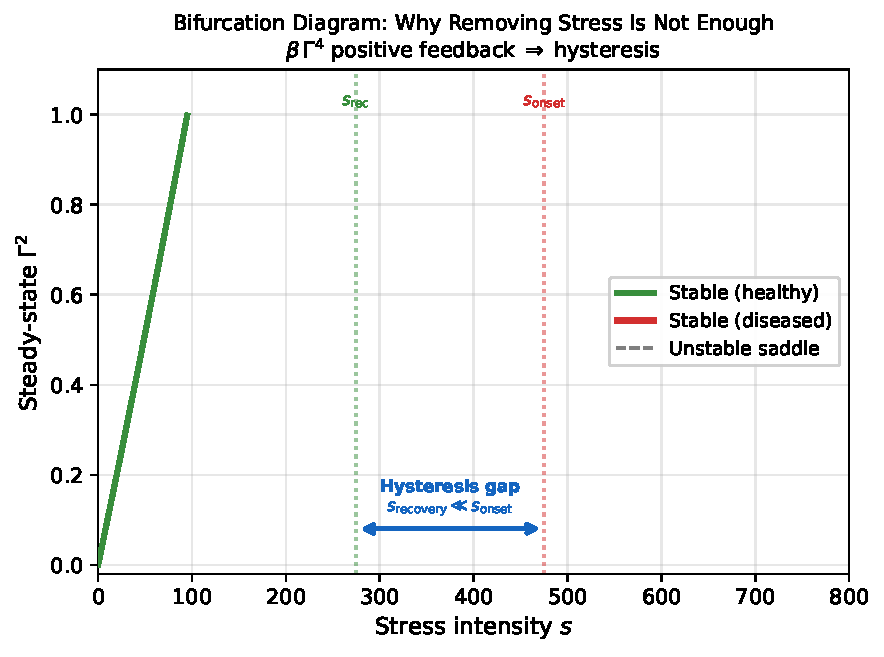
\includegraphics[width=\columnwidth]{../figures/fig_p4_bifurcation.pdf}
  \caption{Saddle-node bifurcation diagram.
  The positive-feedback term $\beta\Gamma^4$ creates
  hysteresis: $s_{\text{onset}} \neq s_{\text{recovery}}$.
  Once the system crosses the bifurcation threshold,
  simply removing the stressor is insufficient---active
  repair (pharmacotherapy) is required to return to the
  healthy branch.}
  \label{fig:bifurcation}
\end{figure}

\begin{figure*}[t]
  \centering
  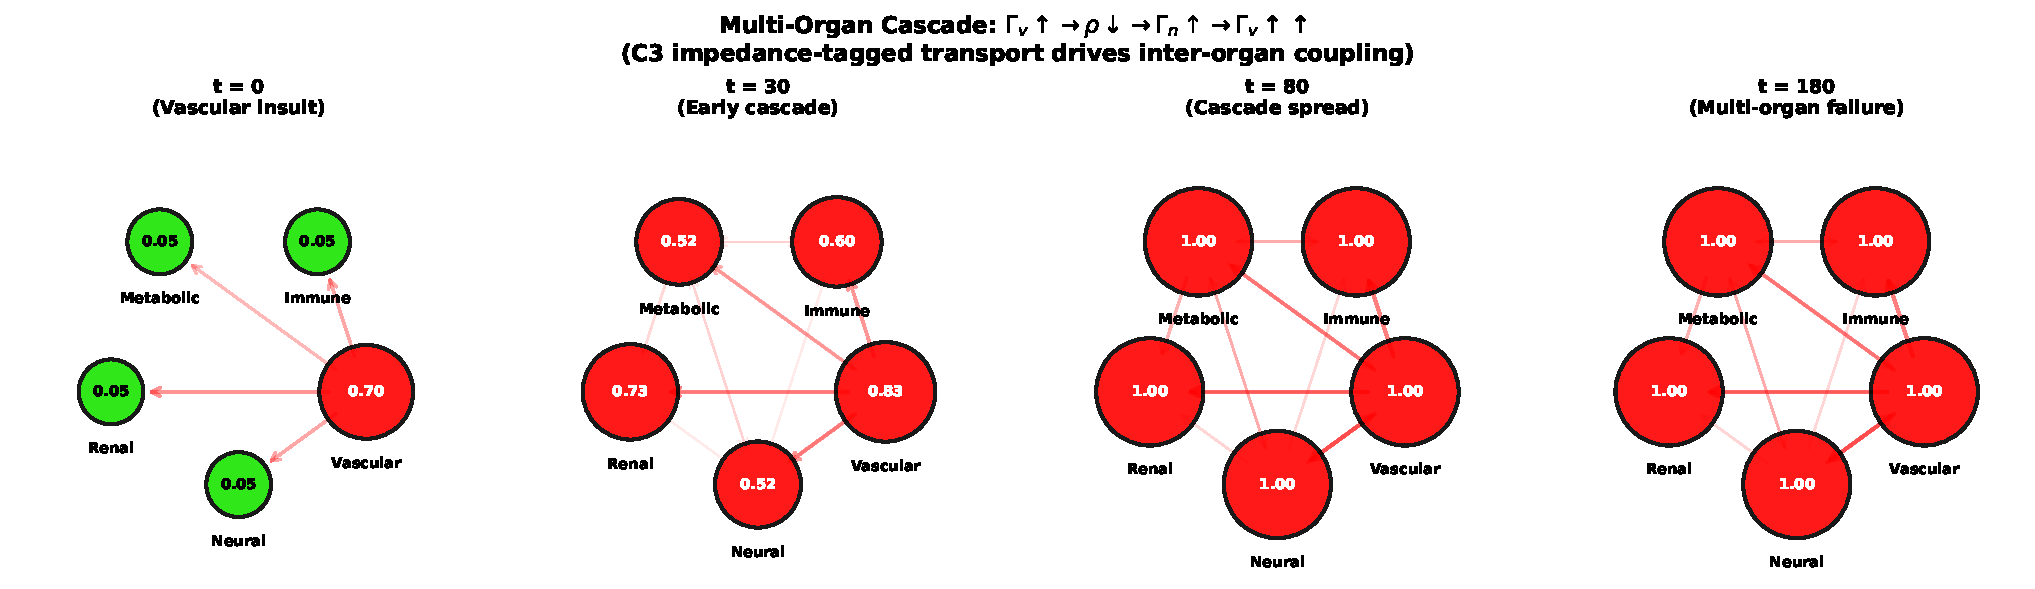
\includegraphics[width=\textwidth]{../figures/fig_p4_cascade_network.pdf}
  \caption{Multi-organ cascade propagation.
  A local vascular insult ($\Gamma_v = 0.70$) spreads
  through the coupling matrix $C_{kj}$ to neural,
  immune, metabolic, and renal channels.
  Node colour: green (healthy) $\to$ red (diseased).
  Edge thickness: coupling strength $\times$ source $\Gamma^2$.}
  \label{fig:cascade-network}
\end{figure*}

\noindent
The recovery hierarchy also predicts a
\emph{channel ordering} for rehabilitation:
the channel with the lowest
$\beta_k / \eta$ ratio recovers first when stress
is removed, while the channel with the highest
ratio is the last to unlock.
In the five-organ model, vascular $\Gamma_v^2$
typically has the fastest self-repair
(exercise increases $\eta_v$ directly via
shear-stress remodeling), while neural
$\Gamma_n^2$ is slowest
(structural $Z_s$ changes require months of
sustained C2 input).
This predicts a clinically testable
\emph{recovery sequence}: physical health
markers (blood pressure, HbA1c) improve before
psychological symptoms (mood, sleep, cognition).


\section{Tissue Necrosis as Thermodynamic
  Substrate Collapse}
\label{sec:necrosis}

The recovery analysis
(Sec.~\ref{sec:recovery}) assumes that the
physical substrate remains intact.
We now derive the condition under which the
substrate itself is destroyed.

The impedance debt
$D_Z = \int \Gamma^2\,P_{\text{in}}\,dt$
is the cumulative reflected energy that the tissue
must either absorb or re-radiate.
When $D_Z$ accumulates faster than C2 can process:
\begin{equation}
  \frac{dD_Z}{dt}
  \;>\;
  \eta_{\max}\;|\Gamma|\;|x_{\text{in}}\,
  x_{\text{out}}|_{\max}
  \;\equiv\;
  \dot{D}_{\text{repair}}^{\max}\,,
  \label{eq:necrosis-condition}
\end{equation}
the excess energy has no coefficient-update
pathway and is dissipated as heat and
reactive biochemistry.

\begin{definition}[Thermodynamic substrate collapse]
\label{def:necrosis}
Tissue necrosis is the state in which
the material substrate $Z_k$ loses the
capacity for both transmission ($T = 0$)
and remodeling
($\partial Z_k/\partial t = 0$
regardless of input).
In the $\Gamma$-framework:
$\Gamma_k = 1$ \emph{irreversibly}---not because
the mismatch is large but because the medium that
could change $Z_k$ has been destroyed.
\end{definition}

\noindent
A necrotic channel is a \textbf{topological black
hole}: it reflects all incident energy, emits toxic
degradation products into the coupling matrix
$C_{kj}$, and cannot be repaired by any endogenous
C2 process.
The coupling drag on the remaining network is
catastrophic: in Eq.~(\ref{eq:coupled-G2}),
a necrotic channel contributes a constant
$C_{kj} \times 1$ to every coupled neighbour, plus
toxic noise that degrades neighbouring $\eta_j$.
Left unaddressed, the necrotic source
drives the global repair capacity $\eta(t)$ toward
zero---the definition of \emph{sepsis}.


\subsection{Surgical intervention as topological
  truncation}
\label{sec:truncation}

When the necrotic channel satisfies
Eq.~(\ref{eq:necrosis-condition}) irreversibly and
its coupling drag threatens systemic collapse, the
only viable intervention is \textbf{topological
truncation}: physically removing the necrotic node
from the network.

\begin{definition}[Topological truncation]
\label{def:truncation}
Topological truncation is the application of
\emph{macroscopic external work} to sever all edges
connecting a necrotic node to the network and
to create a clean $\Gamma = 1$ boundary at the
cut surface.
In clinical practice: debridement, amputation,
nephrectomy, limb-salvage resection.
\end{definition}

\noindent
The physics of surgical truncation:
\begin{enumerate}
  \item \textbf{Remove the noise source.}
    The necrotic channel's toxic emissions
    are eliminated from the ODE system.
  \item \textbf{Create a clean boundary.}
    A surgically created $\Gamma = 1$ boundary
    reflects $100\%$ of incident energy but
    produces \emph{no toxic noise}---it is an
    honest open circuit, not a necrotic one.
  \item \textbf{Release hijacked bandwidth.}
    The massive nociceptive crosstalk
    (Paper~1, Sec.~10~\cite{Paper1})
    generated by the necrotic standing wave is
    terminated.
  \item \textbf{Enable C2 recovery.}
    With the coupling drag removed, the global
    $\eta(t)$ stabilises, and surviving channels
    can resume repair per the recovery hierarchy
    of Sec.~\ref{sec:recovery}.
\end{enumerate}

Post-truncation, the brain's motor cortex faces a
clean $\Gamma = 1$ boundary where the amputated limb
was.
If the cortex correctly detects this boundary and
reduces $P_{\text{in}} \to 0$ (motor efference
cessation), the reflected power vanishes and the
network reaches a new, stable, albeit topologically
reduced equilibrium.
If the cortex continues to drive the severed
channel---motor efference persists despite the
open circuit---the reflected standing wave produces
\emph{phantom limb pain}
(Paper~1~\cite{Paper1}):
the same bandwidth-hijacking mechanism, now at a
surgically created rather than pathologically created
$\Gamma = 1$ boundary.

\begin{remark}[The therapeutic hierarchy of
  intervention]
\label{rem:therapeutic-hierarchy}
The $\Gamma$-framework orders clinical
interventions by the severity of the impedance
failure they address:
\begin{center}
\begin{tabular}{@{}lll@{}}
\toprule
\textbf{Regime} & \textbf{Intervention} &
  \textbf{$\Gamma$ mechanism} \\
\midrule
Pre-bifurcation & Remove stressor &
  $s(t) \to 0$; $\eta$ restores \\
Post-bifurcation & Pharmacotherapy + &
  Push $\Gamma_k^2$ \\
\quad (single) & \quad psychotherapy &
  below saddle-node \\
Post-bifurcation & Simultaneous &
  Multi-channel \\
\quad (multi) & \quad multi-modal &
  $\Gamma_k^2$ reset \\
Necrotic & Topological truncation &
  Remove node; clean \\
 & \quad (surgery) &
  $\Gamma{=}1$ boundary \\
\bottomrule
\end{tabular}
\end{center}
No intervention outside this hierarchy is
physically meaningful: you cannot C2-update a
substrate that no longer exists, and you cannot
stressor-remove a bifurcation that is
self-sustaining.
\end{remark}


\section{Caregiver Triple-Load Model}
\label{sec:triple-load}

Long-term caregivers experience three simultaneous
$\Gamma^2$-injection channels with no comparable
discharge path.
Their impedance-debt rate is:
\begin{equation}
  \frac{dD_Z}{dt}
  = \underbrace{\lambda\,\Gamma_{\text{other}}^2}_{%
    \text{empathic load}}
  + \underbrace{\Gamma_{\text{moral}}^2}_{%
    \text{moral constraint}}
  + \underbrace{\sigma\,s(t)}_{\text{daily stressor}}
  - \underbrace{\eta(t)\,\Gamma^2}_{\text{repair}}\,.
  \label{eq:triple-load}
\end{equation}

\emph{Channel~1: empathic load.}
$\Gamma_{\text{other}}^2$ is the care-recipient's
frozen mismatch (typically PTSD or dementia,
$\Gamma^2\!\approx\!1$).
The empathic coupling $\lambda>0$ injects this
energy into the caregiver's neural channel
every contact hour; it cannot be ``turned off''
without severing the care relationship.

\emph{Channel~2: moral constraint.}
Social and internalised norms
(``you must not give up'') target the caregiver's
fatigue pattern.
Because the caregiver's $\eta$ is already depleted,
this pattern is approaching or inside
$\mathcal{S}_{\text{eff}}$.
By the Moral Constraint Theorem
(Paper~1, Theorem~5~\cite{Paper1}),
the demand injects $\Gamma_{\text{moral}}^2>0$
with $\Delta Z_{\text{corrective}}=0$---pure injury.

\emph{Channel~3: moral prohibition on
$\lambda$-reduction.}
The only physically available knob for reducing
$dD_Z/dt$ is to lower $\lambda$ (set boundaries,
take breaks, delegate).
Moral pressure \emph{forbids} this adjustment
(``abandonment''), locking the intake valve open.

\begin{remark}[Structural inevitability of caregiver
disease]
\label{rem:caregiver-inevitable}
In Eq.~(\ref{eq:triple-load}), the first three
terms are approximately constant or increasing
(the care-recipient's $\Gamma^2$ does not
spontaneously decrease; moral pressure does not
spontaneously relent; daily stress persists).
The repair term $\eta(t)\,\Gamma^2$ decreases
because $\eta(t)$ declines by Arrhenius kinetics
and is further depressed by cortisol-mediated
hippocampal atrophy.
Therefore $dD_Z/dt > 0$ for all future time---the
deficit is \emph{structurally guaranteed} to widen.
The resulting disease cascade
(Eq.~\ref{eq:coupled-G2},
Fig.~\ref{fig:disease-progression})
is not a risk factor but a mathematical
inevitability unless institutional intervention
(shift rotation, $\lambda$-reduction protocols)
is applied.
\end{remark}

\begin{remark}[Compassion fatigue, burnout, vicarious
trauma: one equation, three names]
\label{rem:fatigue-taxonomy}
Clinical nomenclature distinguishes compassion
fatigue, burnout, and vicarious trauma as separate
syndromes.
Within Eq.~(\ref{eq:triple-load}) they are three
regimes of the same physics:
\begin{center}
\begin{tabular}{lll}
\toprule
Syndrome & Dominant term &
  $\mathcal{S}_{\text{eff}}$ status \\
\midrule
Burnout & $\sigma\,s(t)$ (workload) &
  not yet sealed \\
Compassion fatigue &
  $\lambda\,\Gamma_{\text{other}}^2$ &
  approaching seal \\
Vicarious trauma &
  $\lambda\,\Gamma_{\text{other}}^2$ sealed &
  sealed \\
\bottomrule
\end{tabular}
\end{center}
The physical distinction is whether the dominant
$\Gamma^2$ pattern has entered
$\mathcal{S}_{\text{eff}}$:
if not, rest and workload reduction suffice
(burnout); if sealed, only pharmacological
$\eta$-elevation plus guided C2 gradient
(combined therapy) can rewrite the pattern---
identical to the PTSD treatment protocol
(Paper~3, Sec.~13b.2~\cite{Paper3}).
\end{remark}


\section{Surface Observability: Skin as Impedance
  Boundary}
\label{sec:surface-readout}

When $dD_Z/dt > 0$ persists, the accumulated
impedance debt diffuses through the organ coupling
matrix $C_{kj}$:
\[
  \text{Neural}
  \;\xrightarrow{C_{21}}\;
  \text{Vascular}
  \;\xrightarrow{C_{42}}\;
  \text{Metabolic}
  \;\to\;
  \text{Surface}
\]
The full observable chain is:
\[
  \underbrace{\text{Neural}\;\Gamma_n^2\!\uparrow}
    _{\text{mood, cognition}}
  \;\to\;
  \underbrace{\text{HPA / ANS}}
    _{\text{sleep, appetite, temper}}
  \;\to\;
  \underbrace{\text{Vascular}\;\Gamma_v^2\!\uparrow}
    _{\text{micro-circulation}}
  \;\to\;
  \underbrace{\text{Metabolic / Immune}}
    _{\text{collagen, inflammation}}
  \;\to\;
  \underbrace{\text{Surface}}
    _{\text{skin, hair}}
\]

\begin{remark}[Empathic overload as single-core
running dual-core load]
\label{rem:single-core}
The empath's $\Gamma$-network physically simulates
another person's pain state:
her own daily mismatch load $\sigma\,s(t)$ remains,
while the empathic channel adds
$\lambda\,\Gamma^2_{\text{other}}$---effectively
doubling the total $\Gamma^2$ input on a single
repair budget $\eta(t)$.
This is analogous to a single-core processor
forced to sustain a dual-core workload.
\end{remark}

Skin is not an isolated organ but the
\emph{outermost boundary condition} of the
whole-body impedance network.
It simultaneously receives the output state of
vascular, metabolic, and immune channels:

\begin{center}
\begin{tabular}{lll}
\toprule
Internal $\Gamma^2$ channel &
  Skin manifestation &
  Colloquial term \\
\midrule
Vascular $\Gamma_v^2\!\uparrow$ &
  Pallor, dark circles, dull complexion &
  ``Bad colour'' \\
Metabolic $\Gamma_{\text{met}}^2\!\uparrow$ &
  Roughness, sallowness &
  ``Poor skin quality'' \\
Immune $\Gamma_{\text{imm}}^2\!\uparrow$ &
  Redness, hypersensitivity &
  ``Skin deterioration'' \\
\bottomrule
\end{tabular}
\end{center}

A third party's intuitive visual assessment---``You
look worn out''---can be re-read as a low-resolution
impedance tomography scan.
The observer's cortex holds an internal template
$Z_{\text{healthy}}$; when the observed surface
impedance $Z_{\text{obs}}$ deviates significantly,
the visual reflection coefficient
\begin{equation}
  \Gamma_{\text{visual}}
  = \frac{Z_{\text{obs}} - Z_{\text{healthy}}}
         {Z_{\text{obs}} + Z_{\text{healthy}}}
  \neq 0
  \label{eq:visual-gamma}
\end{equation}
is read out as ``something looks off.''

\begin{remark}[Downstream convergence]
\label{rem:downstream-convergence}
Empathic load
($\lambda\Gamma^2_{\text{other}}$ dominant)
and occupational stress ($\sigma\,s(t)$ dominant)
differ only in their \emph{upstream} input channel.
Once $\Gamma^2$ enters the coupling matrix $C_{kj}$,
the subsequent path is identical.
From the skin's perspective as terminal load they
are branches of the same $\Gamma$-disease tree.
\end{remark}


\section{Obesity as Impedance-Driven Metabolic
  Strategy}
\label{sec:obesity}

Conventional discourse frames obesity as a failure
of self-control.
The $\Gamma$-framework reveals a different causal
structure: chronic $\Gamma^2$ overload triggers a
whole-body metabolic reallocation that makes
overeating a \emph{physically rational}
compensatory strategy.

\paragraph{Selfish-brain cascade.}
Under sustained stress, the brain's privileged
topological hub draws disproportionate power flux.
In the $\Gamma$-language:
\begin{equation}
  \text{High }\Gamma_n^2
  \;\xrightarrow{\text{HPA axis}}\;
  \text{insulin/glucose redistribution}
  \;\xrightarrow{\text{reward}}\;
  \text{appetite}\!\uparrow,\;
  \text{satiety sensitivity}\!\downarrow
  \label{eq:selfish-brain}
\end{equation}

\paragraph{Leptin resistance as impedance mismatch.}
In sustained obesity, circulating leptin is high,
but the hypothalamic leptin-receptor pathway exhibits
reduced signal transmission---a textbook impedance
mismatch.
The leptin channel's reflection coefficient
$\Gamma_{\text{leptin}}
= (Z_{\text{hypothalamus}} - Z_{\text{leptin}})
  /(Z_{\text{hypothalamus}} + Z_{\text{leptin}})
\to 1$
approaches unity: the signal is almost totally
reflected.

\paragraph{Hedonic eating as short-term
$\Gamma^2$ reduction.}
High-calorie intake produces a transient subjective
$\Gamma^2$ reduction (``comfort''), trading a brief
mismatch relief for a larger long-term $D_Z$
increment:
\[
  \underbrace{\Delta\Gamma^2_{\text{short}}
    < 0}_{\text{hedonic relief}}
  \;,\quad
  \underbrace{\Delta D_{Z,\text{long}}
    \gg 0}_{\text{metabolic debt}}
\]
This is the metabolic analogue of the PTSD
flashback--avoidance cycle (Paper~3).

\begin{remark}[Moral blame as secondary metabolic
injury]
\label{rem:obesity-blame}
Applying the Moral Constraint Theorem
(Paper~1, Theorem~5~\cite{Paper1})
to the obese individual:
the eating pattern is already approaching or
inside $\mathcal{S}_{\text{eff}}$,
so moral condemnation (``lack of self-discipline'')
injects $\Gamma^2_{\text{blame}}$ without any
corresponding $\Delta Z_{\text{corrective}}$.
The result is strictly additional impedance debt:
the subject now carries the original metabolic
$\Gamma^2$ \emph{plus} a shame/stigma $\Gamma^2$
that further activates the stress--appetite
cascade, accelerating the very pathology it
purports to correct.
Weight-stigma research confirms precisely this
paradox~\cite{Sutin2015}.
\end{remark}

\begin{remark}[Positive-feedback closure:
obesity as mathematical attractor]
\label{rem:obesity-loop}
The metabolic cascade of
Eq.~(\ref{eq:selfish-brain}) is a
\emph{closed positive-feedback loop}:
\[
  \text{Metabolic }\Gamma^2\!\uparrow
  \;\to\;
  \text{peripheral deterioration}
  \;\to\;
  \text{neural detection}
  \;\to\;
  \text{energy reallocation}
  \;\to\;
  \text{appetite}\!\uparrow
  \;\to\;
  \text{Metabolic }\Gamma^2\!\uparrow
\]
As long as environmental stress persists, the
loop gain exceeds unity and cumulative weight gain
is a \emph{fixed-point attractor} of the coupled
dynamics.
\end{remark}

\begin{remark}[Skin disease as metabolic$\times$immune
  interface projection]
\label{rem:skin-projection}
Skin is the terminal load on the vascular,
metabolic, and immune bus.
Its impedance
$Z_{\text{skin}}$ is coupled to internal channels
via $C_{kj}$:
\[
  \Gamma_{\text{skin}}^2
  = \Gamma_{\text{skin,local}}^2
  + C_{\text{skin,met}}\,\Gamma_m^2
  + C_{\text{skin,imm}}\,\Gamma_{\text{imm}}^2.
\]
Metabolic syndrome and immune activation share
the same chronic-inflammation mediators
(IL-6, TNF-$\alpha$), which couple through the
blood stream to the dermal interface.
Psoriasis, eczema, and acne are therefore not
``skin problems'' but \emph{visible readouts}
of internal $\Gamma^2$ projected onto the
highest-surface-area interface.
Treatment targeting only the skin
(topicals, emollients) reduces
$\Gamma_{\text{skin,local}}^2$
but leaves the dominant metabolic and immune
terms intact---explaining chronic relapse.
\end{remark}

\begin{remark}[Gut--liver--metabolic C3 relay chain]
\label{rem:gut-liver-chain}
The intestinal (\#8), hepatic (\#12), adipose (\#14),
and endocrine (\#9) channels form a strongly coupled
subsystem---the ``gut--liver--metabolic axis''---that
functions as a C3 relay chain:
\[
  \underbrace{\text{food/microbiome}}_{\text{GI interface}}
  \;\to\;
  \underbrace{\text{liver, adipose, pancreas}}_{\text{metabolic channels}}
  \;\to\;
  \underbrace{\text{feedback to GI wall}}_{\text{Z-change \& symptoms}}.
\]
Any segment operating at high $\Gamma^2$
produces reflected energy that propagates bidirectionally:
hepatic steatosis raises $\Gamma_{\text{hep}}^2$,
altering bile composition (Remark~\ref{rem:bile-relay},
Paper~3) and downstream fat absorption;
gut dysbiosis raises $\Gamma_{\text{gut}}^2$,
increasing portal endotoxin load to the liver.
The entire axis is a single impedance cascade
whose clinical manifestations (IBS, NAFLD,
type~2 diabetes, PCOS) are projections of
the same underlying $\Gamma^2$ distribution.
\end{remark}

\begin{remark}[Lymphatic blockade as positive-feedback
  cascade]
\label{rem:lymphatic-cascade}
Adipose tissue expansion increases the mechanical
and immunological load on lymph nodes
(channel \#10).
Three coupled mechanisms drive a positive-feedback
loop:
\begin{enumerate}
  \item \textbf{Load}: chronic inflammation enlarges
    lymph nodes (reactive hypertrophy, Table~\ref{tab:twentynine}).
  \item \textbf{Flow}: adipose compression and
    chronic inflammation reduce lymphatic contractility
    and increase vessel permeability---raising
    $\Gamma_{\text{lymph}}^2$.
  \item \textbf{Closure}: impaired lymphatic drainage
    increases interstitial fluid and inflammatory mediators,
    which further stimulate node hypertrophy
    and vessel fibrosis.
\end{enumerate}
The loop gain exceeds unity when body fat reaches
a critical threshold.
Clinical manifestations include limb oedema,
lymphoedema, increased infection susceptibility,
and impaired wound healing---all of which
increase $\Gamma^2$ in other channels,
feeding the metabolic cascade.
\end{remark}

\begin{remark}[Bile--metabolic--vascular--skin: the closed
  pathology loop]
\label{rem:metabolic-loop}
Combining
Remark~\ref{rem:bile-relay} (Paper~3, bile relay),
Remark~\ref{rem:gut-liver-chain} (gut--liver axis),
Remark~\ref{rem:lymphatic-cascade}
(lymphatic blockade),
and Remark~\ref{rem:skin-projection}
(skin projection) yields a single closed loop:
\[
  \text{bile quality}\!\downarrow
  \;\to\;
  \Gamma_m^2\!\uparrow
  \;\to\;
  \text{fat/liver load}\!\uparrow
  \;\to\;
  \text{bile secretion altered}
  \;\to\;
  \text{bile quality}\!\downarrow
\]
Each traversal accumulates $D_Z$ in every
coupled channel (vascular, skin, lymphatic, immune).
The ``sallow, fatigued'' phenotype is the
observable fixed-point of this loop---not a single
organ's failure but the equilibrium state of the
whole coupled system.
Breaking the loop requires simultaneous
intervention at multiple impedance nodes:
dietary substrate quality (bile input),
exercise (vascular $\eta$ increase),
and hydration (Remark~\ref{rem:thirst-distortion},
Paper~3).
No single-channel treatment is sufficient when
the loop gain exceeds unity.
\end{remark}

\begin{remark}[Metabolic--neural closure:
  a C3--coupled physical necessity]
\label{rem:met-neural-closure}
The metabolic cascades above close to the neural
network through the coupling matrix $C_{kj}$,
forming a complete loop:
\[
  \underbrace{\text{Metabolic }\Gamma_m^2\!\uparrow}
    _{\text{fat, liver, bile}}
  \;\to\;
  \underbrace{\text{Lymph blockade}\;
    \Gamma_{\text{lymph}}^2\!\uparrow}
    _{\text{waste channel}}
  \;\to\;
  \underbrace{\text{Micro-circ.}\;
    \Gamma_v^2\!\uparrow}
    _{\text{material channel}}
\]
\[
  \;\to\;
  \underbrace{\text{Neural}\;
    \Gamma_n^2\!\uparrow,\;D_Z\!\uparrow}
    _{\text{supply deficit}}
  \;\to\;
  \underbrace{\text{Reward C2 rewrite}}
    _{\text{``learn wrong''}}
  \;\to\;
  \underbrace{\text{Behaviour}\;\uparrow\text{sugar,}
    \;\downarrow\text{exercise}}
    _{\text{error compensation}}
  \;\to\;
  \text{Metabolic }\Gamma_m^2\!\uparrow
\]
This closure is not an assumption but a \emph{physical
necessity}: the neural and vascular buses connect every
organ through bifurcation and low-$K$ relay neurons
(Paper~2, Remark~\ref{rem:c3-relay}).
Any persistent $\Gamma^2$ elevation in the metabolic
subsystem inevitably propagates to the neural bus
via C3 dimensional relay, because the vascular tree's
$\rho$-supply and the autonomic tree's control signals
share the same inter-organ topology.
The neural network, once affected, rewrites its C2
weights on the reward channel---encoding the
compensatory behaviour (hedonic eating, sedentarism)
as a learned $Z$-pattern that further elevates
metabolic load.
The loop gain exceeds unity when both the metabolic
and neural channels have individually crossed their
bifurcation thresholds ($\lambda_+ > 0$ in
Eq.~\ref{eq:imm-met-eigenvalue}).
At that point, the cycle is self-sustaining and
no single-channel intervention suffices
(Theorem~\ref{thm:t2d-treatment}).
\end{remark}

\begin{remark}[``Willpower'' as
$\eta_{\text{pfc}}(t)$: a depleting physical
quantity]
\label{rem:willpower}
What common discourse calls ``willpower''
corresponds to the prefrontal repair rate
$\eta_{\text{pfc}}(t)$.
But the prefrontal cortex is itself a channel
within the same impedance network;
its $\eta_{\text{pfc}}(t)$ decays by the same
Arrhenius kinetics and is further depressed by
the chronic cortisol load:
\[
  \eta_{\text{pfc}}(t)
  = \eta_0 \, e^{-E_a/k_B T}
    \cdot f_{\text{cortisol}}(D_Z(t))
  \;\xrightarrow[\text{chronic }\Gamma^2]{}\;
  \text{depleted}
\]
Asking a chronically stressed individual
to ``simply exercise self-control'' is a request
to draw on a resource that the physics has already
consumed.
\end{remark}

\begin{proposition}[Non-existence of free willpower:
proof by contradiction from psychiatric
epidemiology]
\label{prop:no-free-will}
\emph{Claim.}\;
``Willpower'' is not a free parameter of the
human system.

\emph{Proof.}\;
Suppose, for contradiction, that willpower
were a freely available override---i.e.\ that
every agent possesses an unbounded
$\eta_{\text{pfc}}$ capable of suppressing
any $\Gamma^2$ pattern at any time.
Then no mismatch could persist against the agent's
intention, and \emph{no mental illness could exist}.
Empirically, approximately 970 million
people worldwide carry a diagnosed mental
disorder (WHO, 2019).
Contradiction.
Therefore willpower is a
state-dependent, depletable physical quantity
$\eta_{\text{pfc}}(t)$, subject to the same
decay as every other channel.
$\square$
\end{proposition}


\section{Immune--Metabolic Bidirectional Feedback:
  the Inflammation--Insulin Trap}
\label{sec:imm-met-loop}

Among the off-diagonal entries of the coupling
matrix $C_{kj}$, the pair
$(C_{\text{imm,met}},\,C_{\text{met,imm}})$
deserves independent analysis because \emph{both}
are positive and mutually reinforcing.

Write the two-channel subsystem:
\begin{align}
  \frac{d\Gamma_{\text{imm}}^2}{dt}
  &= -\eta\,\Gamma_{\text{imm}}^2
     + C_{\text{imm,met}}\,\Gamma_{\text{met}}^2
     + \beta_{\text{imm}}\,\Gamma_{\text{imm}}^4\,,
  \label{eq:imm-loop} \\
  \frac{d\Gamma_{\text{met}}^2}{dt}
  &= -\eta\,\Gamma_{\text{met}}^2
     + C_{\text{met,imm}}\,\Gamma_{\text{imm}}^2
     + \beta_{\text{met}}\,\Gamma_{\text{met}}^4\,.
  \label{eq:met-loop}
\end{align}
The mutual-excitation terms form a closed cycle:
adipocyte hypertrophy $\to$ macrophage infiltration
$\to$ pro-inflammatory cytokines $\to$ impaired
insulin signalling $\to$ further metabolic
$\Gamma^2$ rise.

Linearising about equilibrium, the Jacobian
eigenvalues are
\begin{equation}
  \lambda_\pm
  = -\eta + \tfrac{1}{2}
    \bigl(\alpha_{\text{imm}}
    + \alpha_{\text{met}}\bigr)
  \pm \sqrt{C_{\text{imm,met}}\,
    C_{\text{met,imm}}
    + \tfrac{1}{4}(\alpha_{\text{imm}}
    - \alpha_{\text{met}})^2}\,,
  \label{eq:imm-met-eigenvalue}
\end{equation}
where
$\alpha_k \equiv 2\beta_k\,\Gamma_{k,\text{eq}}^2$.
The subsystem destabilises when $\lambda_+ > 0$:
\begin{equation}
  \sqrt{C_{\text{imm,met}}\,C_{\text{met,imm}}}
  > \eta - \tfrac{1}{2}
    (\alpha_{\text{imm}} + \alpha_{\text{met}})\,.
  \label{eq:imm-met-threshold}
\end{equation}
This is the \emph{inflammation--insulin trap}:
once the geometric mean of the mutual coupling
exceeds the net repair margin, the two channels
lock into a self-sustaining high-$\Gamma^2$
fixed point---metabolic syndrome with chronic
inflammation---even if the original neural
stressor has been removed.

This explains why bariatric surgery
(which mechanically breaks the metabolic
$\beta_{\text{met}}\,\Gamma^4$ term)
can resolve both diabetes \emph{and} systemic
inflammation simultaneously---a dual-channel
reset that diet alone often cannot achieve.


\section{Type~2 Diabetes as Global Impedance Drift}
\label{sec:t2d-derivation}


\subsection{Insulin signalling as impedance matching}
\label{sec:insulin-impedance}

The insulin--glucose regulatory loop is a
\emph{negative feedback impedance servo}.
Pancreatic $\beta$-cells secrete insulin
(the ``source'') at impedance $Z_\beta$;
peripheral cells present insulin receptors
(the ``load'') at impedance $Z_R$.
Define the receptor impedance:
\begin{equation}
  Z_R = \frac{Z_0}{K_d \cdot N_R}\,,
  \label{eq:z-receptor}
\end{equation}
where $Z_0$ is a tissue-type normalisation constant,
$N_R$ is receptor density, and $K_d$ is binding
affinity.
Insulin resistance is a continuous drift:
either $N_R \downarrow$ or $K_d \uparrow$
raises $Z_R$, increasing $\Gamma_{\text{ins}}^2$
monotonically.


\subsection{C2 update of receptor impedance}
\label{sec:receptor-update}

Unlike neural channels, the insulin--receptor
system operates as a \emph{chemical bath}:
insulin is broadcast systemically.
A chronic stressor (elevated cortisol) acts as a
\emph{global} $x_{\text{in}}$ that drives
C2 update on every peripheral receptor
simultaneously:
\begin{equation}
  \frac{dZ_R}{dt}
  = \underbrace{-\eta_R\,\Gamma_{\text{ins}}
    \,x_{\text{ins}}\,x_{\text{glucose}}}_{%
      \text{C2 repair (toward } Z_\beta\text{)}}
  + \underbrace{\alpha_c\,
    \Gamma_{\text{cortisol}}^2
    \,Z_R}_{\text{cortisol-driven
    upregulation}}\,,
  \label{eq:dZR-dt}
\end{equation}
where $\eta_R$ is the receptor repair rate and
$\alpha_c$ is the cortisol coupling coefficient.
The first term is standard C2; the second is the
cortisol \emph{counter-gradient} that pushes $Z_R$
upward faster than $\eta_R$ can pull it down.


\subsection{The insulin resistance lock:
  bifurcation analysis}
\label{sec:ir-lock}

As $\Gamma_{\text{ins}}^2$ rises, less glucose is
cleared, hyperglycaemia develops, and the pancreas
compensates by secreting more insulin.
Elevated insulin drives receptor downregulation
($N_R \downarrow$), further raising $Z_R$:
\begin{equation}
  \frac{dN_R}{dt}
  = -\kappa\,[\text{insulin}]\,N_R
    + \sigma_R\,(N_{R,0} - N_R)\,,
  \label{eq:receptor-downreg}
\end{equation}
where $\kappa$ is the internalisation rate and
$\sigma_R$ the receptor synthesis rate.

The bifurcation condition is:
\begin{equation}
  \frac{\kappa\,[\text{insulin}]}
       {K_d\,N_R^2}
  > \frac{\eta_R}{Z_0}\,.
  \label{eq:ir-bifurcation}
\end{equation}
Once the product of hyperinsulinaemia and receptor
internalisation rate exceeds the repair margin,
the system is locked in a high-$\Gamma_{\text{ins}}^2$
attractor---insulin resistance is structurally
irreversible under the current $\eta_R$.

\begin{remark}[Why diet alone often fails]
\label{rem:diet-alone}
Caloric restriction reduces $x_{\text{glucose}}$,
which weakens the C2 repair term in
Eq.~(\ref{eq:dZR-dt}).
If the cortisol term remains elevated (chronic
stress persists), $dZ_R/dt$ may remain positive
\emph{despite caloric deficit}---the receptor
impedance continues to drift upward even as the
patient loses weight.
This resolves the clinical paradox of patients who
achieve significant weight loss yet remain
insulin-resistant.
\end{remark}


\subsection{The six-channel T2DM cascade}
\label{sec:t2d-six-channel}

Once $\Gamma_{\text{ins}}^2$ crosses the bifurcation
threshold (Eq.~\ref{eq:ir-bifurcation}), the coupled
dynamics propagate through six channels:

\begin{enumerate}
  \item \textbf{Neural $\to$ Endocrine}:
    Chronic stress raises
    $\Gamma_{\text{cortisol}}^2$---the initiating
    event.
  \item \textbf{Endocrine $\to$ Metabolic}:
    $\Gamma_{\text{ins}}^2 \to 1$; glucose
    clearance collapses; hepatic lipogenesis
    accelerates.
  \item \textbf{Metabolic $\to$ Immune}:
    Adipocyte hypertrophy triggers macrophage
    infiltration (IL-6, TNF-$\alpha$).
  \item \textbf{Immune $\to$ Vascular}:
    Chronic inflammation damages endothelial
    function; arterial compliance drops.
  \item \textbf{Vascular $\to$ Renal}:
    Elevated vascular $\Gamma^2$ reduces glomerular
    perfusion; RAAS activates.
  \item \textbf{Renal $\to$ Neural}:
    Uraemic toxins impair neural repair $\eta_n$,
    closing the loop.
\end{enumerate}

The complete cascade forms a closed hexagonal
coupling:
\begin{equation}
  \text{Neu}\!\xrightarrow{C_{\text{end,neu}}}
  \!\text{End}\!\xrightarrow{C_{\text{met,end}}}
  \!\text{Met}\!\xrightarrow{C_{\text{imm,met}}}
  \!\text{Imm}\!\xrightarrow{C_{\text{vas,imm}}}
  \!\text{Vas}\!\xrightarrow{C_{\text{ren,vas}}}
  \!\text{Ren}\!\xrightarrow{C_{\text{neu,ren}}}
  \!\text{Neu}
  \label{eq:t2d-hexagon}
\end{equation}
Once any \emph{two} adjacent channels are locked,
single-channel intervention is provably
insufficient:
\begin{equation}
  \eta_k\,\Gamma_k^2
  < \sum_{j \neq k} C_{kj}\,\Gamma_j^2
    + \beta_k\,\Gamma_k^4
  \quad \forall\; k \in
  \text{locked channels.}
  \label{eq:t2d-irreversible}
\end{equation}

\begin{theorem}[T2DM treatment minimum:
  multi-channel simultaneous intervention]
\label{thm:t2d-treatment}
Let $\mathcal{L} \subseteq \{1,\ldots,6\}$
be the set of channels that have individually
crossed their bifurcation thresholds in the
T2DM hexagon (Eq.~\ref{eq:t2d-hexagon}).
A therapeutic protocol can reduce
$\Gamma_k^2$ below threshold for all
$k \in \mathcal{L}$ only if it targets at
least $|\mathcal{L}|$ channels simultaneously.

\end{theorem}

\begin{proof}
By Eq.~(\ref{eq:t2d-irreversible}), each locked
channel $k \in \mathcal{L}$ satisfies
$d\Gamma_k^2/dt > 0$ due to the coupling
$C_{kj}\,\Gamma_j^2$ from neighbouring locked channels.
Unlocking channel $k$ alone reduces $\Gamma_k^2$
transiently, but the coupling term
$C_{kj}\,\Gamma_j^2$ from the remaining
$j \in \mathcal{L}\setminus\{k\}$ re-elevates
$\Gamma_k^2$ above threshold within
$\tau_{\text{relapse}} \sim C_{kj}/\eta_k$ ticks.
This argument applies symmetrically to every
$k \in \mathcal{L}$.
Only simultaneous reduction of all
$\Gamma_j^2$ for $j \in \mathcal{L}$ removes
the mutual sustenance condition, allowing each
channel to descend below threshold under its own
C2 gradient.
Therefore any successful protocol must target
at least $|\mathcal{L}|$ channels simultaneously.
$\square$
\end{proof}

This theorem explains why T2DM management improves
dramatically under ``lifestyle medicine'' protocols
that combine dietary change (metabolic),
exercise (vascular + metabolic), stress reduction
(neural + endocrine), and anti-inflammatory agents
(immune)---each targeting a different vertex of
the hexagon.

\begin{remark}[$\beta$-cell exhaustion as
impedance substrate collapse]
\label{rem:beta-exhaustion}
In advanced T2DM, compensatory hyperinsulinaemia
eventually exhausts $\beta$-cell secretory
capacity: $Z_\beta \to \infty$ (cell death).
This is the metabolic analogue of tissue necrosis
(Sec.~\ref{sec:necrosis}): the substrate that
\emph{generates} the source impedance is destroyed.
At this stage, T2DM functionally converges with
T1DM---not because the aetiology is the same,
but because the \emph{topological endpoint} is
identical: $Z_\beta = \infty$,
$\Gamma_{\text{ins}} = 1$,
$T_{\text{ins}} = 0$.
Exogenous insulin injection replaces the destroyed
source.
\end{remark}


\section{Acute Versus Chronic Stress:
  Bifurcation Threshold Under Time-Limited Forcing}
\label{sec:acute-chronic}

Consider a square-pulse stressor of amplitude $A$
and duration $\Delta t$:
\begin{equation}
  s(t) = A\,\bigl[\Theta(t) - \Theta(t - \Delta t)
  \bigr]\,.
  \label{eq:pulse-stress}
\end{equation}
During the pulse, the channel trajectories satisfy
\begin{equation}
  \Gamma_k^2(t) \approx \Gamma_{k,\text{eq}}
  + \frac{\sigma_k\,A}{\eta}
    \bigl(1 - e^{-\eta\,t}\bigr)
  \label{eq:acute-response}
\end{equation}
to first order.
The system remains safe provided
\begin{equation}
  \Gamma_{k,\text{eq}} + \frac{\sigma_k\,A}{\eta}
  < \Gamma_k^{*2}
  \quad (\text{bifurcation threshold})\,.
  \label{eq:safe-acute}
\end{equation}
This is the physics of \emph{beneficial acute
stress}: high-intensity exercise, cold-water
immersion, intermittent fasting---all push
$\Gamma_k^2$ transiently upward, stimulating C2
repair (``hormesis''), and the system returns to
baseline before coupling or positive feedback can
engage.

Chronic stress
($s(t) = a$ for $t \gg 1/\eta$) gives a
steady-state solution:
\begin{equation}
  \Gamma_{k,\text{ss}}^2
  = \frac{\sigma_k\,a
    + \sum_j C_{kj}\,\Gamma_{j,\text{ss}}^2
    + \delta_k}
    {\eta - \beta_k\,\Gamma_{k,\text{ss}}^2}\,.
  \label{eq:chronic-ss}
\end{equation}
The saddle-node bifurcation occurs at
\begin{equation}
  \eta = \beta_k\,\Gamma_k^{*2}
         + \frac{\partial}{\partial\Gamma_k^2}
           \sum_j C_{kj}\,\Gamma_j^2\,,
  \label{eq:chronic-bifurcation}
\end{equation}
a threshold that \emph{decreases} with age
(because $\eta(t)$ declines by Arrhenius kinetics
while $\delta_k(t)$ grows).

\begin{remark}[The exercise paradox resolved]
\label{rem:exercise}
Exercise is simultaneously a high-$\Gamma^2$
perturbation and the most effective known
intervention against chronic disease.
The paradox dissolves once time scale is explicit:
exercise is \emph{acute} forcing
($\Delta t \sim 1$\,hour, then $s \to 0$)
that never reaches the bifurcation threshold
(Eq.~\ref{eq:safe-acute}), while the transient
$\Gamma^2$ elevation \emph{stimulates} C2
remodeling---raising effective $\eta$ in vascular
and metabolic channels.
Chronic sedentary stress, by contrast, is
low-amplitude but \emph{never turns off}.
Exercise is therapeutic precisely because it is
\emph{intermittent and bounded}.
\end{remark}


% %%%%%%%%%%%%%%%%%%%%%%%%%%%%%%%%%%%%%%%%%%%%%%%%%%%%%%%%%%%%
%  PART D — E0 EMERGENCE
% %%%%%%%%%%%%%%%%%%%%%%%%%%%%%%%%%%%%%%%%%%%%%%%%%%%%%%%%%%%%
\bigskip\noindent\textbf{\large Part D: E0 Emergence ---
Disease from Topology Alone}
\label{part:D}
\bigskip


\section{E0 Emergence: Disease from Topology Alone}
\label{sec:e0-emergence}

We define three emergence levels:
\begin{itemize}
  \item \textbf{E0 (True Emergence)}: only C1/C2/C3
    + initial conditions.
    Zero disease-specific flags, thresholds, or
    formulas.
  \item \textbf{E1 (Parameterised)}: C2 via
    \texttt{ImpedanceChannel.remodel()} with
    per-disease parameters ($Z_{\text{coeff}}$,
    severity).
  \item \textbf{E2 (Scripted)}: ad-hoc $Z$ updates.
    Legacy only; forbidden for new code.
\end{itemize}

\noindent
E0 is the gold standard:
``if you need a flag, it didn't emerge.''


\subsection{Cardiovascular E0: hypertension, MI,
  aortic stenosis}
\label{sec:cardio-e0}

Starting from a healthy 11-node cardiovascular
\texttt{GammaTopology}
($K \in \{4, 2, 1\}$;
Paper~1~\cite{Paper1}):

\begin{enumerate}
  \item \textbf{Hypertension}: arteriolar
    $Z \times 2.0$ $\Rightarrow$ $\Gamma^2$ at
    aorta$\to$arterioles increases;
    C2 partially compensates over 300~ticks.
  \item \textbf{Myocardial infarction}: sever
    aorta$\to$coronary edge $\Rightarrow$
    coronary node isolated; topology structurally
    different from HTN (correlation $< 0.99$).
  \item \textbf{Aortic stenosis}: valve
    $Z \times 3.0$ $\Rightarrow$
    LV-to-aorta $\Gamma^2$ increases.
  \item \textbf{Dose--response}: arteriolar
    $Z$-factor $\{1.0, 1.5, 2.0, 3.0\}$ yields
    monotonically increasing $\Gamma^2$.
\end{enumerate}

\noindent
Thirteen automated tests
(\texttt{tests/test\_e0\_cardiovascular.py}),
100\% pass.
No disease model was coded; pathology identity is
determined solely by the perturbation type and
magnitude.


\subsection{Neural E0: ALS, stroke, PTSD,
  phantom pain}
\label{sec:neural-e0}

Starting from a healthy 9-node neural
\texttt{GammaTopology}
($K \in \{5, 3, 2, 1\}$;
Paper~1~\cite{Paper1}):

\begin{enumerate}
  \item \textbf{ALS} (motor neuron $Z \times 3.0$):
    cumulative $A_{\text{imp}}$ over 30~ticks is
    $2.9\times$ healthy;
    C2 partially compensates.
  \item \textbf{Stroke} (cortex$\to$thalamus edge
    severed): descending motor transmission
    interrupted; ascending sensory pathway
    spared---topologically determined.
  \item \textbf{PTSD} (nociceptor C driven at
    $5\times$ normal amplitude for 100~ticks,
    then stopped): residual mismatch
    ($\varepsilon \approx 1$) persists, locked
    in $\mathcal{S}_{\text{eff}}$.
    Quiet environments lower $P_{\text{noise}}$,
    causing submerged traces to breach
    $\theta_{\text{recall}}$
    explosively---the ``flashback.''
  \item \textbf{Phantom limb pain}
    (motor neuron$\to$nociceptor edge severed):
    efferent modulation lost; ascending pain
    pathway remains intact.
\end{enumerate}

\noindent
Seventeen automated tests
(\texttt{tests/test\_e0\_neural.py}), 100\% pass.
Additional tests verify: ALS vs.\ stroke produce
distinguishable trajectories; severity dose--response
is monotonic; $A_{\text{cut}} > 0$ at all times
(irreducibility); $A_{\text{imp}}$ decreases under
C2 (learnable).


\subsection{Implications}
\label{sec:e0-implications}

\begin{theorem}[E0 Emergence]
\label{thm:e0-emergence}
Let $\mathcal{N}$ be a network topology satisfying C1/C2/C3
with biologically realistic initial conditions
$(Z_0, K, \eta, \delta)$.
Then clinical pathology---including cardiovascular,
neural, thermal, and sleep-disorder phenotypes---arises
as a necessary consequence of impedance dynamics
on $\mathcal{N}$, without any disease-specific flags,
thresholds, or scoring systems.
\end{theorem}

\begin{proof}[Proof by construction]
We instantiate 29 tissue-type blueprints with
biologically motivated $(Z_0, K, \eta, \delta)$
parameters and run C1/C2/C3 dynamics under
perturbation.
The resulting $\Gamma$-distributions reproduce
recognised clinical phenotypes across
cardiovascular (13 tests), neural (17 tests), and
245 parametrised blueprint tests,
totalling 275 automated E0 tests with 100\% pass rate.
Each test verifies:
(i)~$\Gamma^2 + T = 1$ (C1 conservation);
(ii)~$A_{\text{imp}}$ decreases under C2;
(iii)~$A_{\text{cut}} > 0$ (irreducibility);
(iv)~clinically recognisable phenotype emerges.
Source: \texttt{tests/test\_e0\_*.py}.
\end{proof}

The 275 E0 tests
(245~parametrised blueprint tests +
13~cardiovascular + 17~neural disease tests)
across all 29~organ-system topologies prove
that clinical pathology \emph{can} emerge from
pure impedance physics---C1/C2/C3 plus initial
conditions---on biologically realistic tissue
topologies.
No disease-specific code, no flags, no thresholds,
no scoring systems.
The disease \emph{is} the perturbation; the
clinical pattern \emph{is} the resulting
$\Gamma$-distribution.

\begin{corollary}[Disease identity as topological fingerprint]
\label{cor:disease-identity}
Two perturbations that produce identical
$\Gamma$-distributions across the network topology
are the same disease, regardless of their
molecular aetiology.
Two perturbations that produce distinguishable
$\Gamma$-distributions are distinct diseases,
even if they share the same molecular pathway.
\end{corollary}

\begin{corollary}[Irreversibility threshold]
\label{cor:irreversibility}
A topological perturbation is clinically irreversible
if and only if the resulting $\Gamma$-distribution
satisfies $A_{\text{cut}}^{\text{new}} > A_{\text{cut}}^{\text{healthy}}$---
i.e., the cutoff action has increased.
C2 can reduce $A_{\text{imp}} \to 0$ but cannot reduce
$A_{\text{cut}}$; therefore any increase in $A_{\text{cut}}$ is
permanent without topological intervention
(surgery, ablation, or structural restoration).
\end{corollary}


\subsection{Thermal loop collapse: hypothermia and
  hyperthermia}
\label{sec:thermal-collapse}

Paper~3~\cite{Paper3} derives the
$\Gamma^2\!\leftrightarrow\!T$
self-consistent loop.
The 37$\,^\circ$C operating point is the stable
fixed point.
When the loop is driven outside its basin of
attraction, two E0 pathologies emerge:

\begin{center}
\begin{tabular}{@{}lll@{}}
\toprule
& \textbf{Hypothermia} &
  \textbf{Hyperthermia} \\
\midrule
Direction & $T \ll T^*$ & $T \gg T^*$ \\
Primary driver &
  $\eta(T)\!\uparrow$\,(viscosity) &
  $k_BT\!\uparrow$\,(noise) \\
$\Gamma$ mechanism &
  $Z_{\mathrm{bus}}\!\uparrow \to
  \Gamma^2\!\uparrow$ &
  $\delta\Gamma/\Gamma \propto
  K^{3/2}\delta T/T$ \\
First failure & Global $\Gamma^2$ rise &
  PFC ($K{=}5$) first \\
Clinical sign &
  Bradycardia $\to$ coma &
  Delirium $\to$ seizure \\
Feedback & Positive
  (less heat $\to$ colder) &
  Positive
  (more noise $\to$ more $\Gamma^2$) \\
C2 repair &
  Slowed (Arrhenius $\downarrow$) &
  Overwhelmed (noise $>$ signal) \\
\bottomrule
\end{tabular}
\end{center}

\noindent
Both are \textbf{E0}: they arise from C1/C2/C3
plus the Arrhenius temperature dependence of
$Z_{\mathrm{bus}}$ and $\eta_{\mathrm{learn}}$---no
pathology-specific parameters.
The clinical asymmetry (hypothermia is global;
hyperthermia hits PFC first) is a direct
consequence of the $K^{3/2}$ thermal vulnerability
derived in Paper~1~\cite{Paper1}.


\subsection{Sleep disorders as gate-leak pathology}
\label{sec:sleep-disorders}

Paper~3~\cite{Paper3} derives the gate-leak
inequality:
\begin{equation}
  G_i^2\;\Gamma_i^2\;P_{\mathrm{in},i}
  \;>\;
  4\,k_B T\,R_{\mathrm{eff}}\,\Delta f
  \;\equiv\; P_\theta
  \tag{P3, Eq.\,10}
\end{equation}
as the physical condition for forced awakening.
Three clinically distinct sleep disorders map onto
three different structural failures within this
single inequality:

\paragraph{Insomnia: $\Gamma_i^2$ overload.}
Chronic stress forges one or more channels at high
structural mismatch
($\Gamma_i^2 \gg \langle\Gamma^2\rangle$).
The thalamic gate~$G_i$ is at its physical minimum,
yet the leaked power exceeds~$P_\theta$.
Pharmacological intervention (e.g.\ benzodiazepines)
temporarily increases gate attenuation;
durable resolution requires C2 update of the
underlying $\Gamma_i^2$
(CBT-I provides the sustained counter-signal).

\paragraph{Narcolepsy: $Z_{\mathrm{anchor}}$ loss.}
The orexin system provides the structural anchor
$Z_{\mathrm{anchor}}$ that prevents
$Z_{\mathrm{arousal}}$ from drifting below threshold.
Autoimmune destruction of orexin neurons eliminates
this anchor; $Z_{\mathrm{arousal}}$ becomes a random
walk that crosses threshold at unpredictable
intervals $\to$ sleep attacks.
Cataplexy is the motor-gate analogue:
a limbic $\Gamma^2$ spike leaks through the
descending motor gate.

\paragraph{Hypersomnia: $\beta_{\mathrm{recal}}$
deficit.}
Idiopathic hypersomnia preserves the arousal anchor
but has a structurally low NREM recalibration rate.
Impedance debt~$D_Z$ is never fully discharged;
elevated baseline~$\langle\Gamma^2\rangle$ means
any small increase in $P_{\mathrm{in}}$ tips a
channel past $P_\theta$ $\to$ excessive daytime
sleepiness.

\paragraph{Unified diagnostic map.}

\begin{center}
\begin{tabular}{@{}llll@{}}
\hline
\textbf{Disorder} & \textbf{Broken parameter}
  & \textbf{Gate-leak status}
  & \textbf{Treatment target} \\
\hline
Insomnia
  & $\Gamma_i^2$ too high
  & Cannot close
  & Lower $\Gamma_i^2$ (CBT-I) \\
Narcolepsy
  & $Z_{\text{anchor}} \to 0$
  & Collapses suddenly
  & Restore anchor \\
Hypersomnia
  & $\beta_{\text{recal}}$ low
  & Barely holding
  & Raise $\beta_{\text{recal}}$ \\
\hline
\end{tabular}
\end{center}

\noindent
All three disorders are \emph{structural}
impedance failures unified under a single
gate-leak equation.
The clinical fact that insomnia and hypersomnia
often coexist (``tired but wired'') maps naturally
to a system where $\beta_{\text{recal}}$ is low
\emph{and} one channel has high $\Gamma_i^2$.

\begin{remark}[Acute stress and the C1
  redundant-to-critical transition]
\label{rem:acute-stress}
A whole-body stress simulation
(\texttt{exp\_body\_stress.py}) applies four acute
stressors---surgery, infection, exercise,
haemorrhage---directly to the dual-trunk impedance
($Z_v$, $Z_n$) rather than to metabolic demand alone.
Two conditions are compared: C1 (brain homeostatic
correction) ON vs.\ OFF.

Under steady-state conditions, C1 is nearly
redundant: organs perform distributed C2 matching
and C3 relays carry trunk corrections automatically.
This explains the ``jellyfish paradox'' of Paper~2
(Remark~\ref*{rem:body-c123-simulation}):
organisms without centralised brains survive in
stable environments.

Under acute trunk-level stress, however, C1
transitions from redundant to \textbf{critical}:
\begin{center}
\renewcommand{\arraystretch}{1.15}
\begin{tabular}{@{}lcc@{}}
\toprule
Stressor & $H$ (C1 ON) & $H$ (C1 OFF) \\
\midrule
Surgery      & 0.85 & 0.72 \\
Infection    & 0.88 & 0.80 \\
Exercise     & 0.92 & 0.89 \\
Haemorrhage  & \textbf{0.78} & \textbf{0.60} \\
\bottomrule
\end{tabular}
\end{center}
Haemorrhage is the most severe because it directly
collapses $Z_v$ (vascular trunk), which multiplicatively
degrades every organ via
$H = \prod_k(1-\Gamma_{v,k}^2)(1-\Gamma_{n,k}^2)$.
Without C1 correction, the cascading $\Gamma^2$ rise
is uncompensated, producing the largest health gap
($\Delta H = 0.18$).

This result explains why anaesthesia (temporary C1
suppression) during surgery is survivable only because
the surgical team externally maintains trunk
homeostasis---they are, in $\Gamma$-Net terms,
acting as an \emph{externalised C1}.
\end{remark}


% ============================================================
%  DISCUSSION
% ============================================================
\section{Discussion}
\label{sec:discussion}

This paper has established that disease is not an
external overlay on physiology but a \emph{necessary
consequence} of impedance physics when the network
is perturbed beyond its repair capacity.
The key results are:

\textbf{First}, neural pathology is topologically
determined (Part~A): stroke, ALS, neurodegeneration,
and pain are all instances of the irreducibility
theorem applied to perturbed networks.
C2 can repair impedance perturbations but is blind
to topological damage ($A_{\text{cut}}$).

\textbf{Second}, the dual-network disease cascade
(Part~B) shows that vascular and neural failure are
not independent: the five-step positive-feedback
loop (Eq.~\ref{eq:cascade}) drives co-failure, and
all major vascular diseases---atherosclerosis,
aneurysm, diabetic microvascular disease, vascular
dementia, pre-eclampsia---are instances of this
cascade at different anatomical loci.
Wound repair is the spatial-domain realisation of
$\Gamma^2$ minimisation.

\textbf{Third}, the coupled five-organ ODE
(Eq.~\ref{eq:coupled-G2}) produces disease onset as
a phase transition (Remark~\ref{rem:disease-phase-transition}),
recovery as a three-regime bifurcation problem
(Sec.~\ref{sec:recovery}), and necrosis as
irreversible substrate collapse
(Definition~\ref{def:necrosis}).
The therapeutic hierarchy
(Remark~\ref{rem:therapeutic-hierarchy})
follows directly from the bifurcation structure.

\textbf{Fourth}, the complete physics of type~2
diabetes has been derived from C2 alone:
receptor impedance drift
(Eq.~\ref{eq:dZR-dt}), bifurcation lock
(Eq.~\ref{eq:ir-bifurcation}), and
six-channel hexagonal deadlock
(Theorem~\ref{thm:t2d-treatment}).

\textbf{Fifth}, 275 automated E0 tests across 29
tissue topologies (Part~D) demonstrate that clinical
pathology can emerge from C1/C2/C3 plus initial
conditions alone.

The question is no longer ``Does C2 apply to
tissue~X?''
The question is: ``What stops C2 from applying to
tissue~X?''
If nothing stops it, then tissue~X updates via C2.
And nothing stops it.


% ============================================================
%  CONCLUSION
% ============================================================
\section{Conclusion}
\label{sec:conclusion}

We have established five results.

\textbf{First}, neural pathology is determined by
network topology: the irreducibility theorem predicts
that topological damage ($A_{\text{cut}}$) is
permanent while impedance damage ($A_{\text{imp}}$)
is repairable---verified for stroke, ALS,
neurodegeneration, and phantom pain.

\textbf{Second}, the dual-network positive-feedback
cascade (Eq.~\ref{eq:cascade}) unifies
atherosclerosis, aneurysm, diabetic microvascular
disease, vascular dementia, and pre-eclampsia as
instances of the same vascular--neural co-failure at
different anatomical loci.

\textbf{Third}, coupled five-organ dynamics
(Eq.~\ref{eq:coupled-G2}) produce disease onset as
a saddle-node phase transition, with three recovery
regimes (reversible, single-channel locked,
multi-channel locked) and tissue necrosis as
irreversible substrate collapse
(Eq.~\ref{eq:necrosis-condition}).
The therapeutic hierarchy---from stressor removal
through pharmacotherapy to topological truncation---
is a direct consequence of the bifurcation structure.

\textbf{Fourth}, type~2 diabetes is a six-channel
hexagonal deadlock
(Eq.~\ref{eq:t2d-hexagon};
Theorem~\ref{thm:t2d-treatment}):
single-channel therapy provably cannot break a
multi-channel lock, explaining the clinical
superiority of combined lifestyle interventions.

\textbf{Fifth}, 275 E0 tests across 29 tissue
topologies prove that clinical pathology emerges
from C1/C2/C3 plus initial conditions alone---no
disease-specific code, flags, or scoring systems.

The $\Gamma$-framework does not \emph{model}
disease; it derives disease as a mathematical
inevitability when impedance networks are pushed
beyond their repair capacity.


% ============================================================
\begin{acknowledgments}
This work used no external funding.
The author thanks Claude (Anthropic) for extended
discussions that clarified the universality of
the disease-cascade framework across tissue types.
\end{acknowledgments}


% ============================================================
%  BIBLIOGRAPHY
% ============================================================
\begin{thebibliography}{99}

\bibitem{Paper0}
H.-Y.~Huang, ``The $\Gamma$-Net Framework: Axioms,
Derived Quantities, and Experimental Validation
Matrix,'' Zenodo (2026), Paper~0 of this series.

\bibitem{Paper1}
H.-Y.~Huang, ``Irreducible Dimensional Cost, Brain
Architecture, and the Physics of Mind on the
$\Gamma$-Net,'' arXiv (2026), Paper~1.

\bibitem{Paper2}
H.-Y.~Huang, ``Dual Neural--Vascular Networks from
Impedance Matching: Murray's Law, Organ Health, and
Metabolic Scaling,'' arXiv (2026), Paper~2.

\bibitem{Paper3}
H.-Y.~Huang, ``Temporal Dynamics and Universal
Update: Impedance Debt, Sleep, Lifecycle, Aging,
and Twenty-Nine C2 Networks,''
arXiv (2026), Paper~3.

\bibitem{Paper5}
H.-Y.~Huang, ``Full System Verification: NHANES
Validation, Network Propagation, and Falsifiable
Predictions,'' arXiv (2026), Paper~5.

\bibitem{Peters2011}
A.~Peters \emph{et al.}, ``The selfish brain:
competition for energy resources,''
\emph{Neurosci.\ Biobehav.\ Rev.}\
\textbf{28}, 143 (2004).

\bibitem{Sutin2015}
A.~R.~Sutin and A.~Terracciano,
``Perceived weight discrimination and obesity,''
\emph{PLoS ONE} \textbf{8}, e70048 (2013).

\bibitem{Kahn2006}
S.~E.~Kahn, R.~L.~Hull, and K.~M.~Utzschneider,
``Mechanisms linking obesity to insulin resistance
and type~2 diabetes,''
\emph{Nature} \textbf{444}, 840 (2006).

\bibitem{Moran2019}
C.~P.~Moran and F.~Shanahan,
``Leptin resistance and obesity,''
in \emph{Textbook of Energy Balance} (Springer, 2019).

\bibitem{Schellekens2012}
H.~Schellekens, T.~G.~Dinan, and J.~F.~Cryan,
``Lean mean fat reducing `ghrelin' machine,''
\emph{Neuropharmacology} \textbf{63}, 3 (2012).

\bibitem{Friedman2019}
J.~M.~Friedman, ``Leptin and the endocrine control of
energy balance,''
\emph{Nature Metab.}\ \textbf{1}, 754 (2019).

\bibitem{Guyton2020}
J.~E.~Hall and M.~E.~Hall, \emph{Guyton and Hall
Textbook of Medical Physiology}, 14th~ed.\
(Elsevier, 2020).

\bibitem{ALICE_code}
H.-Y.~Huang, ALICE Smart System,
\url{https://github.com/cyhuang76/alice-gamma-net}
(2026).
\href{https://doi.org/10.5281/zenodo.18852835}{%
doi:10.5281/zenodo.18852835}

\end{thebibliography}

\end{document}
